\documentclass[11pt]{article} % use larger type; default would be 10pt

\usepackage{graphicx} % support the \includegraphics command and options
\usepackage[margin=1.0in]{geometry}
\usepackage{amssymb}
\usepackage{amsmath}

\title{\textbf{A Deterministically Partitioned Element Method for Hexahedral Geometries}}
\author{Giffin, B.; Wopschall, S.}
\date{}

\begin{document}
\maketitle

\section{Abstract}

$<$ Some light stuff $>$

\section{Introduction}

$<$ Some fluffy stuff $>$

\section{Formulation}

$<$ The good stuff $>$
\\\\
$<$ Discussion of the segment minimization procedure $>$
\\
$<$ Segment minimization derivation $>$
\\\\
$<$ Discussion of the facet minimization procedure $>$
\\
\begin{figure} [!ht]
	\centering
	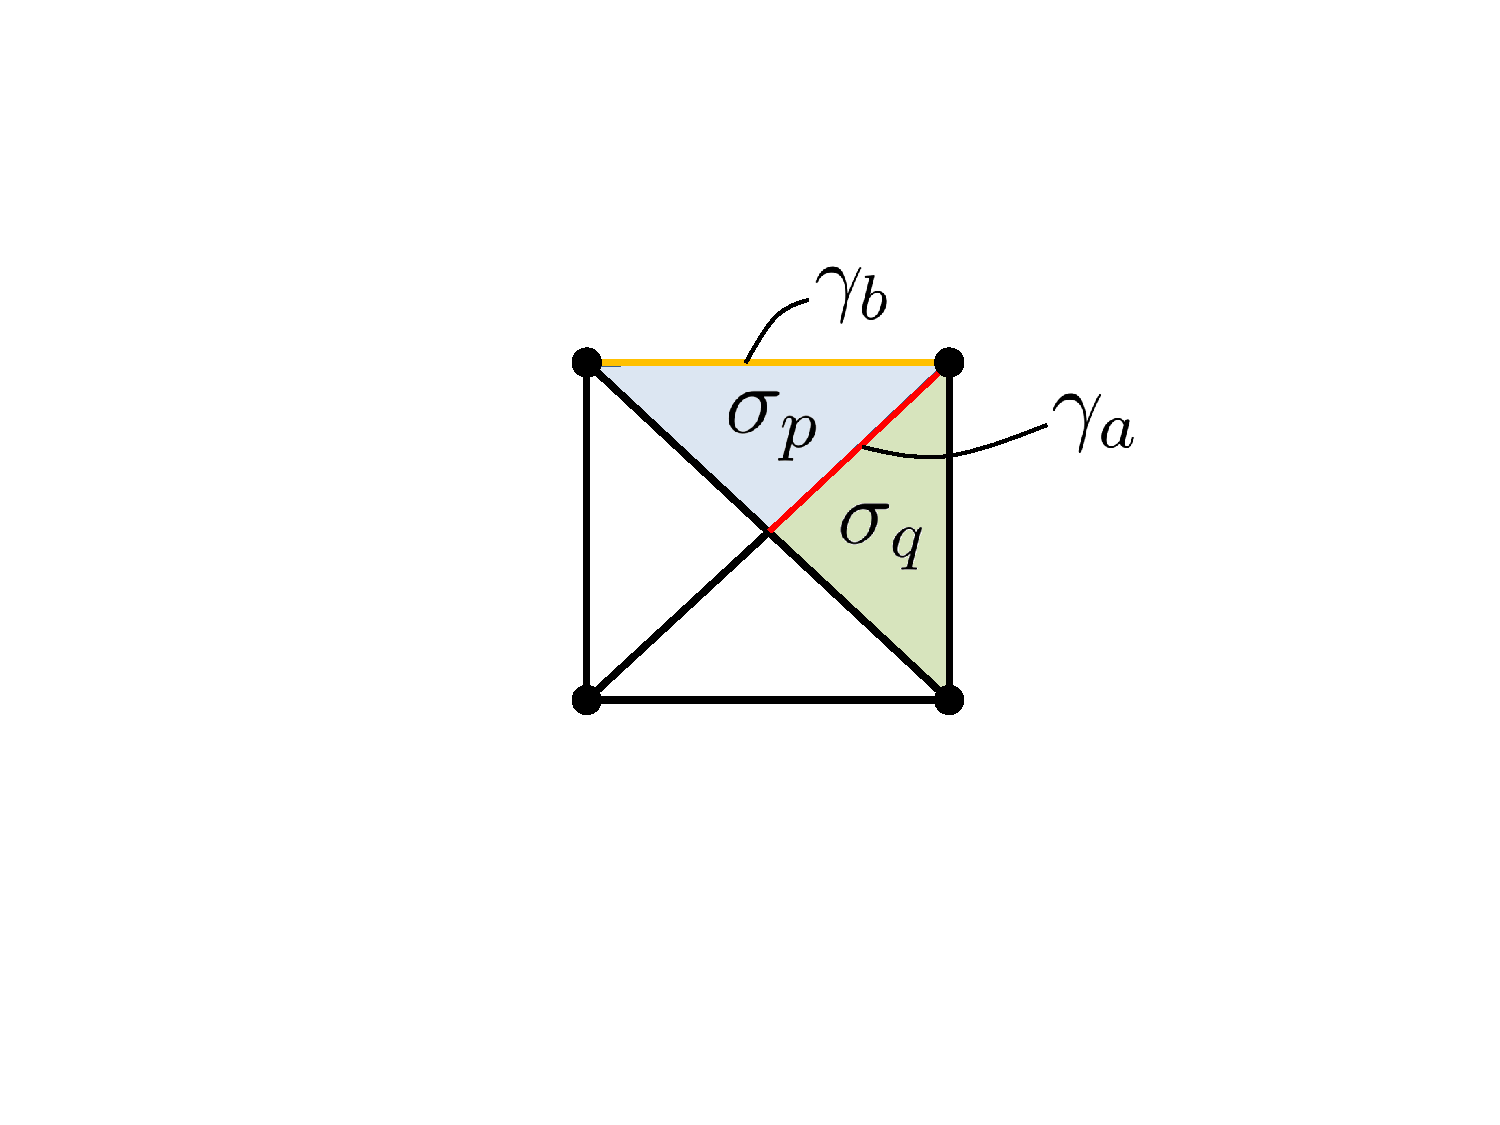
\includegraphics[width = 2.8in,trim=170 190 170 120,clip=true]{facetMinImage.pdf}
	\caption{A representative face of interest.}
	\label{fig:facetMin}
\end{figure}
\begin{center}
\textbf{Facet minimization definitions:}
\end{center}
\begin{itemize}
	\item[$\sigma_p$:] A facet on the current face of interest.
	\item[$| \sigma_p |$:] The area of facet $\sigma_p$.
	\item[$c_p$, $\mathbf{g}_p$:] The unknown (global) coefficients that describe the variation of a particular nodal shape function within facet $p$:
	\begin{equation}
		\varphi_p (\mathbf{x}) = c_p + (\mathbf{x} - \mathbf{x}_p)^T \mathbf{g}_p
	\end{equation}
	\item[$\mathbf{n}_p$:] The outward surface normal of facet $p$.
	\item[$\tilde{\mathbf{g}}_p$:] The unknown (local) gradient coefficients for facet $p$. Note that $\tilde{\mathbf{g}}_p$ is a vector of length 2 with components $\tilde{g}^{(p)}_1$, $\tilde{g}^{(p)}_2$. These could be defined in association with a particular orthonormal basis ($\tilde{\mathbf{e}}^p_1$, $\tilde{\mathbf{e}}^p_2$) such that $\tilde{\mathbf{e}}^p_1 \times \tilde{\mathbf{e}}^p_2 = \mathbf{n}_p$, and $\mathbf{g}_p = \tilde{g}^{(p)}_1 \tilde{\mathbf{e}}^p_1 + \tilde{g}^{(p)}_2 \tilde{\mathbf{e}}^p_2$. Necessarily then, $\mathbf{g}_p \cdot \mathbf{n}_p = 0$. In matrix form, this may be written as:
	\begin{equation}
		\mathbf{g}_p = \mathbf{A}_p \tilde{\mathbf{g}}_p
	\end{equation}
	where in this circumstance,
	\begin{equation}
		\mathbf{A}_p = \left[ \begin{array}{cc} \tilde{\mathbf{e}}^p_1 & \tilde{\mathbf{e}}^p_2 \end{array} \right]
	\end{equation}
	$\mathbf{A}_p$ is therefore a matrix of dimension $3 \times 2$.

	Alternatively, we could impose the constraint $\mathbf{g}_p \cdot \mathbf{n}_p = 0$ by writing one of the global gradient coefficients in terms of the other two, e.g.
	\begin{equation}
		g_3^{(p)} = \frac{-n_1^{(p)} g_1^{(p)} -n_2^{(p)} g_2^{(p)}}{n_3^{(p)}}
	\end{equation}
	This permits $\tilde{\mathbf{g}}_p$ to be chosen such that
	\begin{equation}
		\tilde{\mathbf{g}}_p = \left[ \begin{array}{c} g^{(p)}_1 \\ g^{(p)}_2 \end{array} \right]
	\end{equation}
	and consequently,
	\begin{equation}
		\mathbf{A}_p = \left[ \begin{array}{cc} 1 & 0 \\ 0 & 1 \\ -n_1^{(p)}/n_3^{(p)} & -n_2^{(p)}/n_3^{(p)} \end{array} \right]
	\end{equation}
	In either case, $\mathbf{g}_p$ may be written in terms of only two unknown (local) coefficients for each facet.
	\item[$\mathbf{x}_p$:] An arbitrarily chosen reference position on facet $p$.
	\item[$\mathcal{L}$:] The set of all ``interior'' segments on the current face.
	\item[$\mathcal{B}$:] The set of all ``exterior'' segments on the current face.
	\item[$\gamma_a$:] An ``interior'' segment, such that $a \in \mathcal{L}$; one that borders two facets: $\sigma_p$ and $\sigma_q$.
	\item[$\gamma_b$:] An ``exterior'' segment, such that $b \in \mathcal{B}$; one that borders a single facet: $\sigma_p$.
	\item[$\bar{c}_b$, $\bar{\mathbf{g}}_b$:] The known (global) coefficients that describe the variation of a particular nodal shape function within segment $b$:
	\begin{equation}
		\varphi_b (\mathbf{x}) = \bar{c}_b + (\mathbf{x} - \mathbf{x}_b)^T \bar{\mathbf{g}}_b
	\end{equation}
	\item[$\mathbf{x}_b$:] An arbitrarily chosen reference position on segment $b$.
	\item[$| \gamma_a |$:] The length of segment $\gamma_a$ (similarly for $| \gamma_b |$).
	\item[$\mathbf{n}^{(p)}_a$:] A (local) outward segment normal, constrained to lie in the plane of facet $p$. If $\gamma_a$ has a local parameterization such that $\mathbf{x} (s) = \mathbf{x}_a + s \mathbf{\xi}_a$, then we can determine $\mathbf{n}^{(p)}_a$ via:
	\begin{equation}
		\mathbf{n}^{(p)}_a = \mathbf{\xi}_a \times \mathbf{n}_p
	\end{equation}
	\item[$\varepsilon$:] A measure of the jump in value of a given shape function on interior segments:
	\begin{equation}
		\varepsilon = \varphi_p (\mathbf{x}) - \varphi_q (\mathbf{x})
	\end{equation}
	\begin{equation}
		\varepsilon = c_p + (\mathbf{x} - \mathbf{x}_p)^T \mathbf{g}_p - c_q - (\mathbf{x} - \mathbf{x}_q)^T \mathbf{g}_q
	\end{equation}
	on exterior segments:
	\begin{equation}
		\varepsilon = \varphi_p (\mathbf{x}) - \varphi_b (\mathbf{x})
	\end{equation}
	\begin{equation}
		\varepsilon = c_p + (\mathbf{x} - \mathbf{x}_p)^T \mathbf{g}_p - \bar{c}_b - (\mathbf{x} - \mathbf{x}_b)^T \bar{\mathbf{g}}_b
	\end{equation}
	\item[$\Delta$:] A measure of the jump in normal derivative of a given shape function on interior segments:
	\begin{equation}
		\Delta = {\mathbf{n}^{(p)}_a}^T \nabla \varphi_p (\mathbf{x}) + {\mathbf{n}^{(q)}_a}^T \nabla \varphi_q (\mathbf{x})
	\end{equation}
	\begin{equation}
		\Delta = {\mathbf{n}^{(p)}_a}^T \mathbf{g}_p + {\mathbf{n}^{(q)}_a}^T \mathbf{g}_q
	\end{equation}
	\item[$\beta_2$:] An adjustable parameter, such that $\beta_2 \in (0, 1)$. If $\beta_2 = 0$, $\mathcal{F}$ only penalizes jumps in the normal derivative of the shape function between facets (evaluated on \textit{interior} segments). This effects smoothness of the resulting shape functions. If $\beta_2 = 1$, $\mathcal{F}$ only penalizes jumps in the value of the shape function between facets (evaluated on \textit{interior} segments). This effects continuity of the resulting shape functions (on the interior of the face).
	\item[$\alpha_2$:] Yet another adjustable parameter. If $\alpha_2 > 0$, $\mathcal{F}$ will penalize jumps in the value of the shape function between facets and the boundary of the face (evaluated on \textit{exterior} segments). This effects continuity of the resulting shape functions (on the exterior of the face).
	\item[$\mathcal{F}_2$:] The quadratic functional for a face that is to be minimized with respect to $c_p$ and $\tilde{\mathbf{g}}_p$ for all facets $p$:
	\begin{eqnarray}
	\mathcal{F}_2 = (1-\beta_2) \sum_{a \in \mathcal{L}} | \gamma_a | \int_{\gamma_a} \frac{1}{2} \Delta^2 d \xi + \beta_2 \sum_{a \in \mathcal{L}} \frac{1}{| \gamma_a |} \int_{\gamma_a} \frac{1}{2} \varepsilon^2 d \xi \nonumber \\ + \alpha_2 \sum_{b \in \mathcal{B}} \frac{1}{| \gamma_b |} \int_{\gamma_b} \frac{1}{2} \varepsilon^2 d \xi
\end{eqnarray}
\end{itemize}

\begin{center}
\textbf{Minimization Procedure:}
\end{center}

Now that we have taken care of the relevant definitions, we may elaborate on the minimization procedure. Ultimately, we seek the unknown (local) coefficients $c_p$ and $\tilde{\mathbf{g}}_p$ for all facets $p$. These are obtained via
\begin{equation}
	\min_{c_p, \, \tilde{\mathbf{g}}_p} \mathcal{F} \, \, \forall q
\end{equation}
It proves convenient to look at the minimization associated with only one particular interior segment $\gamma_a$:
\begin{equation}
	\mathcal{F}^a_2 = (1-\beta_2) | \gamma_a | \int_{\gamma_a} \frac{1}{2} \Delta^2 d \xi + \beta_2 \frac{1}{| \gamma_a |} \int_{\gamma_a} \frac{1}{2} \varepsilon^2 d \xi
\end{equation}
\begin{equation}
	\frac{\partial \mathcal{F}^a_2}{\partial c_p} = 0; \qquad \frac{\partial \mathcal{F}^a_2}{\partial \tilde{\mathbf{g}}_p} = \mathbf{0}
\end{equation}
\begin{equation}
	\frac{\partial \mathcal{F}^a_2}{\partial c_q} = 0; \qquad \frac{\partial \mathcal{F}^a_2}{\partial \tilde{\mathbf{g}}_q} = \mathbf{0}
\end{equation}
and one particular exterior segment $\gamma_b$:
\begin{equation}
	\mathcal{F}^b_2 = \alpha_2 \frac{1}{| \gamma_b |} \int_{\gamma_b} \frac{1}{2} \varepsilon^2 d \xi
\end{equation}
\begin{equation}
	\frac{\partial \mathcal{F}^b_2}{\partial c_p} = 0; \qquad \frac{\partial \mathcal{F}^b_2}{\partial \tilde{\mathbf{g}}_p} = \mathbf{0}
\end{equation}

For the interior segment:
\begin{equation}
	\frac{\partial \mathcal{F}^a_2}{\partial c_p} = (1-\beta_2) | \gamma_a | \int_{\gamma_a} \Delta \frac{\partial \Delta}{\partial c_p} d \xi + \beta_2 \frac{1}{| \gamma_a |} \int_{\gamma_a} \varepsilon \frac{\partial \varepsilon}{\partial c_p} d \xi
\end{equation}
\begin{equation}
	\frac{\partial \mathcal{F}^a_2}{\partial \tilde{\mathbf{g}}_p} = (1-\beta_2) | \gamma_a | \int_{\gamma_a} \Delta \frac{\partial \Delta}{\partial \tilde{\mathbf{g}}_p} d \xi + \beta_2 \frac{1}{| \gamma_a |} \int_{\gamma_a} \varepsilon \frac{\partial \varepsilon}{\partial \tilde{\mathbf{g}}_p} d \xi
\end{equation}
\begin{equation}
	\frac{\partial \mathcal{F}^a_2}{\partial c_q} = (1-\beta_2) | \gamma_a | \int_{\gamma_a} \Delta \frac{\partial \Delta}{\partial c_q} d \xi + \beta_2 \frac{1}{| \gamma_a |} \int_{\gamma_a} \varepsilon \frac{\partial \varepsilon}{\partial c_q} d \xi
\end{equation}
\begin{equation}
	\frac{\partial \mathcal{F}^a_2}{\partial \tilde{\mathbf{g}}_q} = (1-\beta_2) | \gamma_a | \int_{\gamma_a} \Delta \frac{\partial \Delta}{\partial \tilde{\mathbf{g}}_q} d \xi + \beta_2 \frac{1}{| \gamma_a |} \int_{\gamma_a} \varepsilon \frac{\partial \varepsilon}{\partial \tilde{\mathbf{g}}_q} d \xi
\end{equation}
Examining terms of interest, and noting that
\begin{equation}
	\frac{\partial \mathbf{g}_p}{\partial \tilde{\mathbf{g}}_p} = \mathbf{A}_p, \quad \frac{\partial \mathbf{g}_q}{\partial \tilde{\mathbf{g}}_q} = \mathbf{A}_q
\end{equation}
we find
\begin{equation}
	\frac{\partial \Delta}{\partial c_p} = 0, \quad \frac{\partial \Delta}{\partial c_q} = 0
\end{equation}
\begin{equation}
	\frac{\partial \varepsilon}{\partial c_p} = 1, \quad \frac{\partial \varepsilon}{\partial c_q} = -1
\end{equation}
\begin{equation}
	\frac{\partial \Delta}{\partial \tilde{\mathbf{g}}_p} = {\mathbf{n}_a^{(p)}}^T \mathbf{A}_p, \quad \frac{\partial \Delta}{\partial \tilde{\mathbf{g}}_q} = {\mathbf{n}_a^{(q)}}^T \mathbf{A}_q
\end{equation}
\begin{equation}
	\frac{\partial \varepsilon}{\partial \tilde{\mathbf{g}}_p} = (\mathbf{x} - \mathbf{x}_p)^T \mathbf{A}_p, \quad \frac{\partial \varepsilon}{\partial \tilde{\mathbf{g}}_q} = -(\mathbf{x} - \mathbf{x}_q)^T \mathbf{A}_q
\end{equation}
Making the appropriate substitutions,
\begin{equation}
	\frac{\partial \mathcal{F}^a_2}{\partial c_p} = \beta_2 \frac{1}{| \gamma_a |} \int_{\gamma_a} \left[ c_p + (\mathbf{x} - \mathbf{x}_p)^T \mathbf{A}_p \tilde{\mathbf{g}}_p - c_q - (\mathbf{x} - \mathbf{x}_q)^T \mathbf{A}_q \tilde{\mathbf{g}}_q \right] d \xi
\end{equation}
\begin{equation}
	\frac{\partial \mathcal{F}^a_2}{\partial c_q} = \beta_2 \frac{1}{| \gamma_a |} \int_{\gamma_a} \left[ -c_p - (\mathbf{x} - \mathbf{x}_p)^T \mathbf{A}_p \tilde{\mathbf{g}}_p + c_q + (\mathbf{x} - \mathbf{x}_q)^T \mathbf{A}_q \tilde{\mathbf{g}}_q \right] d \xi
\end{equation}
\begin{eqnarray}
	\frac{\partial \mathcal{F}^a_2}{\partial \tilde{\mathbf{g}}_p} = (1-\beta_2) | \gamma_a | \int_{\gamma_a} \left[ {\mathbf{n}^{(p)}_a}^T \mathbf{g}_p + {\mathbf{n}^{(q)}_a}^T \mathbf{g}_q \right] {\mathbf{n}_a^{(p)}}^T \mathbf{A}_p d \xi \nonumber \\ + \beta_2 \frac{1}{| \gamma_a |} \int_{\gamma_a} \left[ c_p + (\mathbf{x} - \mathbf{x}_p)^T \mathbf{A}_p \tilde{\mathbf{g}}_p - c_q - (\mathbf{x} - \mathbf{x}_q)^T \mathbf{A}_q \tilde{\mathbf{g}}_q \right] (\mathbf{x} - \mathbf{x}_p)^T \mathbf{A}_p d \xi
\end{eqnarray}
\begin{eqnarray}
	\frac{\partial \mathcal{F}^a_2}{\partial \tilde{\mathbf{g}}_q} = (1-\beta_2) | \gamma_a | \int_{\gamma_a} \left[ {\mathbf{n}^{(p)}_a}^T \mathbf{g}_p + {\mathbf{n}^{(q)}_a}^T \mathbf{g}_q \right] {\mathbf{n}_a^{(q)}}^T \mathbf{A}_q d \xi \nonumber \\ + \beta_2 \frac{1}{| \gamma_a |} \int_{\gamma_a} \left[ -c_p - (\mathbf{x} - \mathbf{x}_p)^T \mathbf{A}_p \tilde{\mathbf{g}}_p + c_q + (\mathbf{x} - \mathbf{x}_q)^T \mathbf{A}_q \tilde{\mathbf{g}}_q \right] (\mathbf{x} - \mathbf{x}_q)^T \mathbf{A}_q d \xi
\end{eqnarray}
If we define the following terms:
\begin{equation}
	k_{cc} = \beta_2 \frac{1}{| \gamma_a |} \int_{\gamma_a} d \xi \quad (1 \times 1)
\end{equation}
\begin{equation}
	\mathbf{k}_{cg}^{(q)} = \beta_2 \frac{1}{| \gamma_a |} \int_{\gamma_a} (\mathbf{x} - \mathbf{x}_q)^T \mathbf{A}_q d \xi \quad (1 \times 2)
\end{equation}
\begin{equation}
	\mathbf{k}_{gc}^{(p)} = \beta_2 \frac{1}{| \gamma_a |} \int_{\gamma_a} \mathbf{A}^T_p (\mathbf{x} - \mathbf{x}_p) d \xi \quad (2 \times 1)
\end{equation}
\begin{eqnarray}
	\mathbf{k}_{gg}^{(p,q)} = \beta_2 \frac{1}{| \gamma_a |} \int_{\gamma_a} \mathbf{A}^T_p (\mathbf{x} - \mathbf{x}_p) (\mathbf{x} - \mathbf{x}_q)^T \mathbf{A}_q d \xi \quad (2 \times 2)
\end{eqnarray}
\begin{eqnarray}
	\hat{\mathbf{k}}_{gg}^{(p,q)} = (1-\beta_2) | \gamma_a | \int_{\gamma_a} \mathbf{A}^T_p {\mathbf{n}_a^{(p)}} {\mathbf{n}^{(q)}_a}^T \mathbf{A}_q d \xi \quad (2 \times 2)
\end{eqnarray}
and if we further define:
\begin{equation}
	\mathbf{K}_{pq}^{(a)} = \left[ \begin{array}{cc} k_{cc} & \mathbf{k}_{cg}^{(q)} \\ \mathbf{k}_{gc}^{(p)} & \mathbf{k}_{gg}^{(p,q)} \end{array} \right] \quad (3 \times 3)
\end{equation}
\begin{equation}
	\hat{\mathbf{K}}_{pq}^{(a)} = \left[ \begin{array}{cc} 0 & \mathbf{0}^T \\ \mathbf{0} & \hat{\mathbf{k}}_{gg}^{(p,q)} \end{array} \right] \quad (3 \times 3)
\end{equation}
\begin{equation}
	\mathbf{u}_p = \left\{ \begin{array}{cc} c_p & \tilde{\mathbf{g}}^T_p \end{array} \right\}^T \quad (3 \times 1)
\end{equation}
then we may recast the local minimization for segment $a$ in the form of a local $6\times6$ contribution to the global minimization problem:
\begin{equation}
	\left[ \begin{array}{cc} (\hat{\mathbf{K}}_{pp}^{(a)} + \mathbf{K}_{pp}^{(a)}) & (\hat{\mathbf{K}}_{pq}^{(a)}-\mathbf{K}_{pq}^{(a)}) \\ (\hat{\mathbf{K}}_{qp}^{(a)}-\mathbf{K}_{qp}^{(a)}) & (\hat{\mathbf{K}}_{qq}^{(a)}+\mathbf{K}_{qq}^{(a)}) \end{array} \right] \left\{ \begin{array}{c} \mathbf{u}_p \\ \mathbf{u}_q \end{array} \right\} = \left\{ \begin{array}{c} \mathbf{0} \\ \mathbf{0} \end{array} \right\}
\end{equation}

We may proceed in a similar manner to determine a local contribution from the exterior segment:
\begin{equation}
	\frac{\partial \mathcal{F}^b_2}{\partial c_p} = \alpha_2 \frac{1}{| \gamma_b |} \int_{\gamma_b} \varepsilon \frac{\partial \varepsilon}{\partial c_p} d \xi
\end{equation}
\begin{equation}
	\frac{\partial \mathcal{F}^b_2}{\partial \tilde{\mathbf{g}}_p} = \alpha_2 \frac{1}{| \gamma_b |} \int_{\gamma_b} \varepsilon \frac{\partial \varepsilon}{\partial \tilde{\mathbf{g}}_p} d \xi
\end{equation}
We recall
\begin{equation}
	\frac{\partial \varepsilon}{\partial c_p} = 1, \quad \frac{\partial \varepsilon}{\partial \tilde{\mathbf{g}}_p} = (\mathbf{x} - \mathbf{x}_p)^T \mathbf{A}_p
\end{equation}
Making the appropriate substitutions,
\begin{equation}
	\frac{\partial \mathcal{F}^b_2}{\partial c_p} = \alpha_2 \frac{1}{| \gamma_b |} \int_{\gamma_b} \left[ c_p + (\mathbf{x} - \mathbf{x}_p)^T \mathbf{A}_p \tilde{\mathbf{g}}_p - \bar{c}_b - (\mathbf{x} - \mathbf{x}_b)^T \bar{\mathbf{g}}_b \right] d \xi
\end{equation}
\begin{eqnarray}
	\frac{\partial \mathcal{F}^b_2}{\partial \tilde{\mathbf{g}}_p} = \alpha_2 \frac{1}{| \gamma_b |} \int_{\gamma_b} \left[ c_p + (\mathbf{x} - \mathbf{x}_p)^T \mathbf{A}_p \tilde{\mathbf{g}}_p - \bar{c}_b - (\mathbf{x} - \mathbf{x}_b)^T \bar{\mathbf{g}}_b \right] (\mathbf{x} - \mathbf{x}_p)^T \mathbf{A}_p d \xi
\end{eqnarray}
If we define the following terms:
\begin{equation}
	\bar{k}_{cc} = \alpha_2 \frac{1}{| \gamma_b |} \int_{\gamma_b} d \xi \quad (1 \times 1)
\end{equation}
\begin{equation}
	\bar{\mathbf{k}}_{cg}^{(p)} = \alpha_2 \frac{1}{| \gamma_b |} \int_{\gamma_b} (\mathbf{x} - \mathbf{x}_p)^T \mathbf{A}_p d \xi \quad (1 \times 2)
\end{equation}
\begin{equation}
	\bar{\mathbf{k}}_{gc}^{(p)} = \left[ \bar{\mathbf{k}}_{cg}^{(p)} \right]^T \quad (2 \times 1)
\end{equation}
\begin{equation}
	\bar{\mathbf{k}}_{cg}^{(b)} = \alpha_2 \frac{1}{| \gamma_b |} \int_{\gamma_b} (\mathbf{x} - \mathbf{x}_b)^T d \xi \quad (1 \times 3)
\end{equation}
\begin{eqnarray}
	\bar{\mathbf{k}}_{gg}^{(p,p)} = \alpha_2 \frac{1}{| \gamma_b |} \int_{\gamma_b} \mathbf{A}^T_p (\mathbf{x} - \mathbf{x}_p) (\mathbf{x} - \mathbf{x}_p)^T \mathbf{A}_p d \xi \quad (2 \times 2)
\end{eqnarray}
\begin{eqnarray}
	\bar{\mathbf{k}}_{gg}^{(p,b)} = \alpha_2 \frac{1}{| \gamma_b |} \int_{\gamma_b} \mathbf{A}^T_p (\mathbf{x} - \mathbf{x}_p) (\mathbf{x} - \mathbf{x}_b)^T d \xi \quad (2 \times 3)
\end{eqnarray}
and if we further define:
\begin{equation}
	\bar{\mathbf{K}}_{pp}^{(b)} = \left[ \begin{array}{cc} \bar{k}_{cc} & \bar{\mathbf{k}}_{cg}^{(p)} \\ \bar{\mathbf{k}}_{gc}^{(p)} & \bar{\mathbf{k}}_{gg}^{(p,p)} \end{array} \right] \quad (3 \times 3)
\end{equation}
\begin{equation}
	\bar{\mathbf{K}}_{pb}^{(b)} = \left[ \begin{array}{cc} \bar{k}_{cc} & \bar{\mathbf{k}}_{cg}^{(b)} \\ \bar{\mathbf{k}}_{gc}^{(p)} & \bar{\mathbf{k}}_{gg}^{(p,b)} \end{array} \right] \quad (3 \times 4)
\end{equation}
\begin{equation}
	\bar{\mathbf{u}}_b = \left\{ \begin{array}{cc} \bar{c}_b & \bar{\mathbf{g}}^T_b \end{array} \right\}^T \quad (4 \times 1)
\end{equation}
\begin{equation}
	\mathbf{f}^{(b)}_p = \bar{\mathbf{K}}_{pb}^{(b)} \bar{\mathbf{u}}_b \quad (3 \times 1)
\end{equation}
then we may recast the local minimization for segment $b$ in the form of a local $3\times3$ contribution to the global minimization problem:
\begin{equation}
	\bar{\mathbf{K}}_{pp}^{(b)} \mathbf{u}_p = \mathbf{f}^{(b)}_p
\end{equation}

\begin{figure} [!ht]
	\centering
	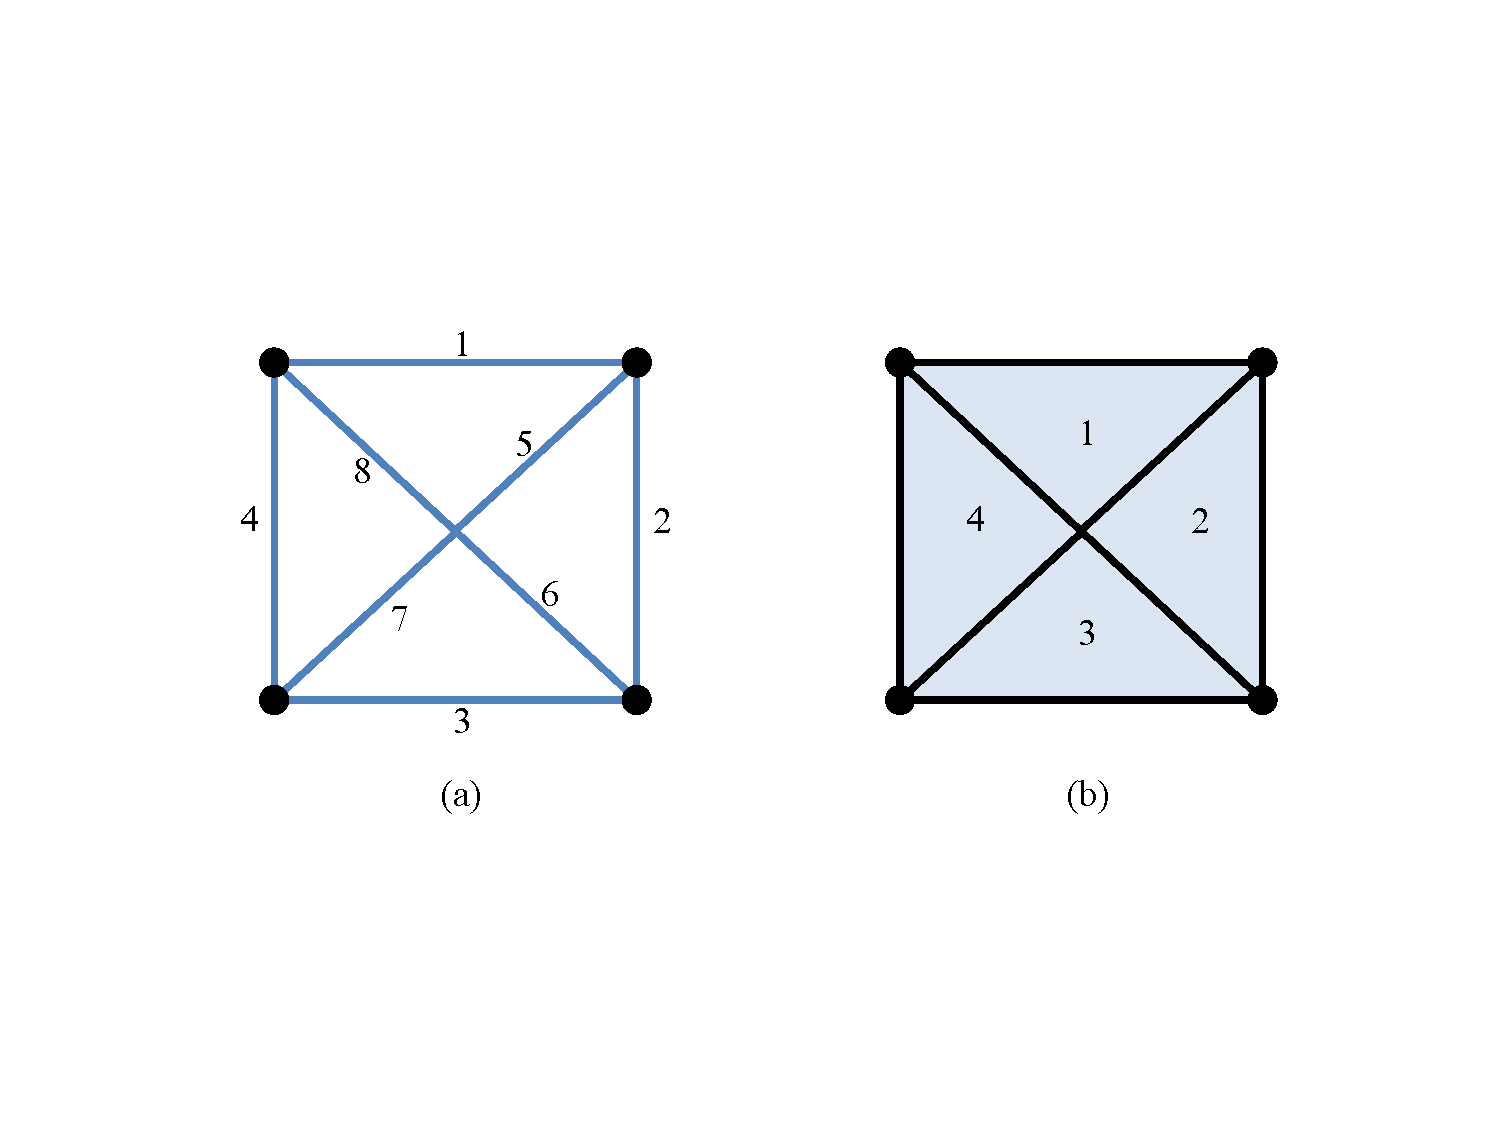
\includegraphics[width = 5in,trim=100 150 100 150,clip=true]{numbering.pdf}
	\caption{Example (a) segment and (b) facet numbering schemes.}
	\label{fig:numbering}
\end{figure}
If we were to assume the segment and facet numbering schemes depicted in Figure \ref{fig:numbering}, then the resulting $12\times12$ system of equations would appear as follows:
\begin{equation}
	\mathbf{K}_2 \mathbf{U}_2 = \mathbf{F}_2
\end{equation}
where
\begin{eqnarray}
	\mathbf{K}_2 = \left[ \begin{array}{cccc} \bar{\mathbf{K}}_{11}^{(1)}+\mathbf{K}_{11}^{(5)}+\mathbf{K}_{11}^{(8)} & -\mathbf{K}_{12}^{(5)} & 0 & -\mathbf{K}_{14}^{(8)} \\ -\mathbf{K}_{21}^{(5)} & \bar{\mathbf{K}}_{22}^{(2)}+\mathbf{K}_{22}^{(5)}+\mathbf{K}_{22}^{(6)} & -\mathbf{K}_{23}^{(6)} & 0 \\ 0 & -\mathbf{K}_{32}^{(6)} & \bar{\mathbf{K}}_{33}^{(3)}+\mathbf{K}_{33}^{(5)}+\mathbf{K}_{33}^{(7)} & -\mathbf{K}_{34}^{(7)} \\ -\mathbf{K}_{41}^{(8)} & 0 & -\mathbf{K}_{43}^{(7)} & \bar{\mathbf{K}}_{44}^{(4)}+\mathbf{K}_{44}^{(5)}+\mathbf{K}_{44}^{(8)} \end{array} \right]
\end{eqnarray}
\begin{equation}
	\mathbf{U}_2 = \left\{ \begin{array}{c} \mathbf{u}_1 \\ \mathbf{u}_2 \\ \mathbf{u}_3 \\ \mathbf{u}_4 \end{array} \right\}, \quad \mathbf{F}_2 = \left\{ \begin{array}{c} \mathbf{f}^{(1)}_1 \\ \mathbf{f}^{(2)}_2 \\ \mathbf{f}^{(3)}_3 \\ \mathbf{f}^{(4)}_4 \end{array} \right\}
\end{equation}
The subscripted $_2$ denotes that we are referring to the system of equations that result from minimizing $\mathcal{F}_2$ (the face minimization problem).

\begin{center}
\textbf{Facet Least Squares Best-Fit Correction:}
\end{center}

Suffice it say, there is no free lunch: the foregoing PEM minimization does not always guarantee linear completeness of the resulting shape functions. In particular, if a face is non-planar, then we must supplement our formulation with a ``least-squares best-fit'' operator (denoted $\bar{\mathbf{Q}}$), which ultimately provides us with linear completeness.

If we suppose that we are given a number of nodal values $\varphi_a$, where $a = 1, \ldots, n$ now denotes a node on the face of interest, and if we know the coordinates of each node $\mathbf{x}_a$, then we would like to determine an average (face-wide) globally linear function $\bar{\varphi} (\mathbf{x})$, such that
\begin{equation}
	\bar{\varphi} (\mathbf{x}) = \bar{c} + (\mathbf{x} - \bar{\mathbf{x}})^T \bar{\mathbf{g}}
\end{equation}
where $\bar{\mathbf{x}}$ is some arbitrarily chosen reference coordinate, preferrably selected to lie on the face in question (though this is not a requirement). Our goal then is to set the global coefficients $\bar{c}$ and $\bar{\mathbf{g}}$ of this function, such that
\begin{equation}
	\min_{(\bar{c}, \bar{\mathbf{g}})} \frac{1}{2} \sum_a w_a \hat{\varphi}_a^2
\end{equation}
where we have defined the ``nodal residual'' at node $a$ to be:
\begin{equation}
	\hat{\varphi}_a = \varphi_a - \bar{\varphi} (\mathbf{x}_a)
\end{equation}
and $w_a$ are minimization weights associated with each node. For simplicity, these weights could all be set equal to $1$. Alternatively, one might choose to determine the weights based on tributary face areas, or edge lengths. Irrespective of the choice of $w_a$, we recognize this minimization to be nothing more than a weighted least-squares best-fit of the nodal values. If we define the following terms (consistent with the canonical linear least-squares literature):
\begin{equation}
	\mathbf{X}_a = \left\{ \begin{array}{cc} 1 & (\mathbf{x}_a - \bar{\mathbf{x}})^T \end{array} \right\} \quad (1\times4)
\end{equation}
\begin{equation}
	\mathbf{X} = \left[ \begin{array}{c} \mathbf{X}_1 \\ \mathbf{X}_2 \\ \vdots \\ \mathbf{X}_n \end{array} \right] \quad (n\times4)
\end{equation}
\begin{equation}
	\mathbf{W} = \left[ \begin{array}{cccc} w_1 & 0 & \cdots & 0 \\ 0 & w_2 & \cdots & 0 \\ \vdots & \vdots & \ddots & \vdots \\ 0 & 0 & \cdots & w_n \end{array} \right] \quad (n\times n)
\end{equation}
\begin{equation}
	\mathbf{y} = \left\{ \begin{array}{c} \varphi_1 \\ \varphi_2 \\ \vdots \\ \varphi_n \end{array} \right\} \quad (n \times 1)
\end{equation}
\begin{equation}
	\mathbf{\beta} = \left\{ \begin{array}{c} \bar{c} \\ \bar{\mathbf{g}} \end{array} \right\} \quad (4 \times 1)
\end{equation}
The resulting global function coefficients may be written as
\begin{equation}
	\mathbf{\beta} = \big( \mathbf{X}^T \mathbf{W} \mathbf{X} \big)^{-1} \mathbf{W} \mathbf{X}^T \mathbf{y}
\end{equation}
If we insist that $\bar{\mathbf{Q}}$ be a mapping of nodal values $\varphi_a$ to the global function coefficients $\bar{c}$ and $\bar{\mathbf{g}}$, then we may write
\begin{equation}
	\bar{\mathbf{Q}} = \big( \mathbf{X}^T \mathbf{W} \mathbf{X} \big)^{-1} \mathbf{W} \mathbf{X}^T \quad (4 \times n)
\end{equation}
This implies that the best-fit function evaluated at $\mathbf{x}_a$ can be expressed as
\begin{equation}
	\bar{\varphi} (\mathbf{x}_a) = \mathbf{X}_a \mathbf{\beta} = \mathbf{X}_a \bar{\mathbf{Q}} \mathbf{y}
\end{equation}

However, implicit in this representation is the fact that the best-fit function refers to some \textit{arbitrarily} chosen reference position on the face, and thus will not necessarily agree with the choice of reference position used for each individual facet. If we were to attempt to compose the face-wide mapping $\bar{\mathbf{Q}}$ with each of the mappings $\mathbf{Q}_p$ for the individual facets, then there would be a discrepancy in the locations of the reference coordinates used in each of the mappings. Specifically, 
\begin{equation}
	\varphi_p (\mathbf{x}) = c_p + (\mathbf{x} - \mathbf{x}_p)^T \mathbf{g}_p \neq \bar{c} + (\mathbf{x} - \bar{\mathbf{x}})^T \bar{\mathbf{g}} = \bar{\varphi} (\mathbf{x})
\end{equation}

If we define the vector of residual nodal values $\hat{\mathbf{y}}$ as
\begin{equation}
	\hat{\mathbf{y}} = \left\{ \begin{array}{c} \hat{\varphi}_1 \\ \hat{\varphi}_2 \\ \vdots \\ \hat{\varphi}_n \end{array} \right\} \quad (n \times 1)
\end{equation}
and if we further define $\hat{\mathbf{Q}}$ as an operator that takes nodal values $\varphi_a$ and maps them to residual nodal values $\hat{\varphi}_a$, i.e.
\begin{equation}
	\hat{\mathbf{Q}} = \mathbf{I} - \mathbf{X} \bar{\mathbf{Q}} \quad (n \times n)
\end{equation}
\begin{equation}
	\hat{\mathbf{y}} = \hat{\mathbf{Q}} \mathbf{y}
\end{equation}
then, for non-planar faces, we would write the corrected global coefficient mappings $\mathbf{Q}_p$ for each facet $p$ of the face as:
\begin{equation}
	\mathbf{Q}_p \leftarrow \bar{\mathbf{Q}} + \mathbf{Q}_p \hat{\mathbf{Q}} \quad (4 \times n)
\end{equation}
The above correction will guarantee linear completeness of the resulting shape functions. However, it should be noted that the $4 \times 4$ matrix $\mathbf{X}^T \mathbf{W} \mathbf{X}$ will be rank deficient (not invertible) if the nodes of a particular face are co-planar. In this circumstance, the least-squares best-fit correction can be omitted, or else the generalized inverse of $\mathbf{X}^T \mathbf{W} \mathbf{X}$ may be used with impunity.

\newpage

\begin{center}
\textbf{Second Order Quadrature Consistency:}
\end{center}

Consider the strong-form of equilibrium in the abscence of body force:
\begin{equation}
	T_{ij,j} = 0 \quad \forall x_i \in B,
\end{equation}
the equivalent weak-form of equilibirum in the abscence of body force:
\begin{equation}
	\int_{\Omega} T_{ij,j} dv = \int_{\Gamma} t_i da \quad \forall \Omega \subset B
\end{equation}
and the Galerkin approximation to the weak form:
\begin{equation}
	\int_{\Omega} T_{ij} \varphi_{a,j} dv = \int_{\Gamma} t_i \varphi_a da = \int_{\Gamma} T_{ij} \varphi_a n_j da \quad \forall a.
\end{equation}
Technically speaking, this last may only hold on element domains, i.e.
\begin{equation}
	\int_{\Omega_e} T_{ij} \varphi_{a,j} dv = \int_{\Gamma_e} T_{ij} \varphi_a n_j da \quad \forall a.
\end{equation}
Let us suppose that the stress field satisfies a linear spatial variation (corresponding to a quadratic displacement field), namely
\begin{equation}
	T_{ij} (x_k) = \bar{T}_{ij} + \bar{T}_{ij,k} x_k,
\end{equation}
such that
\begin{equation}
	\int_{\Omega_e} (\bar{T}_{ij} + \bar{T}_{ij,k} x_k) \varphi_{a,j} dv = \int_{\Gamma_e} (\bar{T}_{ij} + \bar{T}_{ij,k} x_k) \varphi_a n_j da \quad \forall a.
\end{equation}
This implies that
\begin{equation}
	\bar{T}_{ij} \bigg(\int_{\Omega_e} \varphi_{a,j} dv - \int_{\Gamma_e} \varphi_a n_j da \bigg) + \bar{T}_{ij,k} \bigg( \int_{\Omega_e} x_k \varphi_{a,j} dv - \int_{\Gamma_e} x_k \varphi_a n_j da \bigg) = 0  \quad \forall a.
\end{equation}
However, since the displacement field is arbitrary, $\bar{T}_{ij}$ and $\bar{T}_{ij,k}$ are therefore arbitrary, and we require
\begin{equation}
	\int_{\Omega_e} \varphi_{a,j} dv = \int_{\Gamma_e} \varphi_a n_j da \quad \forall a,
\end{equation}
\begin{equation}
	\int_{\Omega_e} x_k \varphi_{a,j} dv = \int_{\Gamma_e} x_k \varphi_a n_j da \quad \forall a.
\end{equation}
These conditions constitute first- and second-order ``quadrature consistency,'' respectively. For PEM elements, this amounts to
\begin{equation}
	\sum_{q} | \omega_q | \varphi_{a,j}^{(q)} = \sum_{\alpha} | \sigma_{\alpha} | n_j^{(\alpha)} \varphi_a^{(\alpha)},
\end{equation}
\begin{equation}
	\sum_{q} | \omega_q | \bar{x}_k^{(q)} \varphi_{a,j}^{(q)} = \sum_{\alpha} | \sigma_{\alpha} | \bar{x}_k^{(\alpha)} n_j^{(\alpha)} \varphi_a^{(\alpha)}.
\end{equation}
This suggests that even if the displacement field itself is not able to exactly reproduce a spatially quadratic field (due to interpolation error), second-order quadrature consistency may still guarantee exact integration of the weak form when the \textit{nodes} are set consistent with such a field. It may well be the case that such elements will exhibit improved convergence in the $H^1$ energy semi-norm, but will otherwise retain second-order convergence in the $L^2$ displacement norm. Improvement in the $L^2$ convergence rate may perhaps be had by further refinement of the element into a greater number of quadrature sub-cells.

\newpage

\begin{center}
\textbf{Integration of Polynomial Expressions on Arbitrary Polytopes:}
\end{center}

Suppose we wish to integrate a polynomial expression $P^{(p)}(\mathbf{x})$ of degree $p$
\begin{equation}
	P^{(p)}(\mathbf{x}) = \sum_{r=0}^{p} a_r \mathbf{x}^r
\end{equation}
over an arbitrary closed $n$-polytope $\Omega_q \subset V$ ($V$ being an isometry of $\mathbb{R}^n$), which itself is embedded in $\mathbb{R}^d$ (such that $\mathbf{x} \in \mathbb{R}^d$). We identify $\mathbf{x}^r$ as a tensor of rank $r$ (e.g. $\mathbf{x}^2 = \mathbf{x} \otimes \mathbf{x}$). We are interested in computing
\begin{equation}
	\int_{\Omega_q} P^{(p)}(\mathbf{x}) d \Omega = \sum_{r=0}^{p} a_r \int_{\Omega_q} \mathbf{x}^r d \Omega,
\end{equation}
meaning we must be able to integrate $\int_{\Omega_q} \mathbf{x}^r d \Omega \, \, \forall r$. Let us suppose that $\mathbf{x}$ may be written as $\mathbf{x} = \mathbf{x}_q + \hat{\mathbf{x}}$, where $\mathbf{x}_q \in \mathbb{R}^d$ is some fixed reference position on the $n$-polytope, and $\hat{\mathbf{x}} \in V$ is variable. Thus,
\begin{equation}
	\int_{\Omega_q} \mathbf{x}^r d \Omega = \int_{\Omega_q} (\mathbf{x}_q + \hat{\mathbf{x}})^r d \Omega = \sum_{k = 0}^r \binom{r}{k} \mathbf{x}_q^{(r-k)} \int_{\Omega_q} \hat{\mathbf{x}}^k d \Omega.
\end{equation}
By the divergence theorem
\begin{equation}
	\int_{\Omega_q} \hat{\mathbf{x}}^k d \Omega = \frac{1}{n+k} \int_{\Gamma} \langle \hat{\mathbf{x}}^{(k+1)} , \mathbf{n} \rangle \, d \Gamma
\end{equation}
where $\Gamma$ constitutes the boundary of $\Omega_q$, and $\mathbf{n} \in V$ is the unit outward normal. If we suppose that $\Gamma = \cup_{\alpha} \Gamma_{\alpha}$, where $\Gamma_{\alpha} \in S_{\alpha}$ are $(n-1)$-polytopes, then we have
\begin{equation}
	\int_{\Omega_q} \hat{\mathbf{x}}^k d \Omega = \frac{1}{n+k} \sum_{\alpha} \mathbf{x}_{\alpha} \cdot \mathbf{n}_{\alpha} \int_{\Gamma_{\alpha}} \hat{\mathbf{x}}^k   d \Gamma
\end{equation}
where we suppose $\hat{\mathbf{x}} = \mathbf{x}_{\alpha} + \hat{\mathbf{x}}_{\alpha}$, $\mathbf{x}_{\alpha} \in V$ is again some fixed reference position on the $(n-1)$-polytope of interest, and $\hat{\mathbf{x}}_{\alpha} \in S_{\alpha}$ is variable. Therefore,
\begin{equation}
	\int_{\Omega_q} \mathbf{x}^r d \Omega = \sum_{k = 0}^r \binom{r}{k} \mathbf{x}_q^{(r-k)} \frac{1}{n+k} \sum_{\alpha} \mathbf{x}_{\alpha} \cdot \mathbf{n}_{\alpha} \int_{\Gamma_{\alpha}} \hat{\mathbf{x}}^k   d \Gamma
\end{equation}
Thus, the 0th, 1st, and 2nd moments are (respectively):
\begin{equation}
	\int_{\Omega_q} d \Omega = \frac{1}{n} \sum_{\alpha} \mathbf{x}_{\alpha} \cdot \mathbf{n}_{\alpha} \int_{\Gamma_{\alpha}} d \Gamma
\end{equation}
\begin{equation}
	\int_{\Omega_q} \mathbf{x} d \Omega = \mathbf{x}_q \int_{\Omega_q} d \Omega + \frac{1}{n+1} \sum_{\alpha} \mathbf{x}_{\alpha} \cdot \mathbf{n}_{\alpha} \int_{\Gamma_{\alpha}} \hat{\mathbf{x}} d \Gamma
\end{equation}
\begin{equation}
	\int_{\Omega_q} \mathbf{x} \otimes \mathbf{x} d \Omega = - \mathbf{x}_q \otimes \mathbf{x}_q \int_{\Omega_q} d \Omega + \mathbf{x}_q \otimes \left[ \int_{\Omega_q} \mathbf{x} d \Omega \right] + \left[ \int_{\Omega_q} \mathbf{x} d \Omega \right] \otimes \mathbf{x}_q + \frac{1}{n+2} \sum_{\alpha} \mathbf{x}_{\alpha} \cdot \mathbf{n}_{\alpha} \int_{\Gamma_{\alpha}} \hat{\mathbf{x}} \otimes \hat{\mathbf{x}} d \Gamma
\end{equation}
Note, however, that
\begin{equation}
	\mathbf{x}_{\alpha} \cdot \mathbf{n}_{\alpha} = (\mathbf{x} - \mathbf{x}_q - \hat{\mathbf{x}}_{\alpha}) \cdot \mathbf{n}_{\alpha} = (\mathbf{x} - \mathbf{x}_q) \cdot \mathbf{n}_{\alpha} =  (\mathbf{a}_{\alpha} - \mathbf{x}_q) \cdot \mathbf{n}_{\alpha}
\end{equation}
\begin{equation}
	\hat{\mathbf{x}} = (\mathbf{x} - \mathbf{x}_q)
\end{equation}
where $\mathbf{x} = \mathbf{a}_{\alpha} + \hat{\mathbf{a}}_{\alpha}$ is yet another shifted coordinate system, and $\mathbf{a}_{\alpha}$ is a fixed reference position on the $(n-1)$-polytope denoted by $\alpha$, being measured from the global origin. Therefore,
\begin{equation}
	\int_{\Omega_q} d \Omega = \frac{1}{n} \left[ \sum_{\alpha} (\mathbf{a}_{\alpha} - \mathbf{x}_q) \cdot \mathbf{n}_{\alpha} \int_{\Gamma_{\alpha}} d \Gamma \right]
\end{equation}
\begin{equation}
	\int_{\Omega_q} \mathbf{x} d \Omega = \frac{1}{n+1} \left[ \mathbf{x}_q \int_{\Omega_q} d \Omega + \sum_{\alpha} (\mathbf{a}_{\alpha} - \mathbf{x}_q) \cdot \mathbf{n}_{\alpha} \int_{\Gamma_{\alpha}} \mathbf{x} d \Gamma \right]
\end{equation}
\begin{equation}
	\int_{\Omega_q} \mathbf{x} \otimes \mathbf{x} d \Omega = \frac{1}{n+2} \left[ \mathbf{x}_q \otimes \int_{\Omega_q} \mathbf{x} d \Omega + \int_{\Omega_q} \mathbf{x} d \Omega \otimes \mathbf{x}_q + \sum_{\alpha} (\mathbf{a}_{\alpha} - \mathbf{x}_q) \cdot \mathbf{n}_{\alpha} \int_{\Gamma_{\alpha}} \mathbf{x} \otimes \mathbf{x} d \Gamma \right]
\end{equation}

Consider now a two-noded segment $\gamma$ whose nodal coordinates are given by $\mathbf{a}_1$ and $\mathbf{a}_2$. The integral evaluations on the segment reduce to simply:
\begin{equation}
	\int_{\gamma} d \gamma \equiv | \gamma | = || \mathbf{a}_{2} - \mathbf{a}_{1} ||
\end{equation}
\begin{equation}
	\int_{\gamma} \mathbf{x} d \gamma = \frac{| \gamma |}{2} (\mathbf{a}_{1} + \mathbf{a}_{2})
\end{equation}
\begin{equation}
	\int_{\gamma} \mathbf{x} \otimes \mathbf{x} d \gamma = \frac{| \gamma |}{6} \left[ 2 (\mathbf{a}_{1} \otimes \mathbf{a}_{1} + \mathbf{a}_{2} \otimes \mathbf{a}_{2}) + \mathbf{a}_{1} \otimes \mathbf{a}_{2} + \mathbf{a}_{2} \otimes \mathbf{a}_{1} \right]
\end{equation}
or, by the parallel axis theorem:
\begin{equation}
	\int_{\gamma} \mathbf{x} \otimes \mathbf{x} d \gamma = \bar{\mathbf{x}} \otimes \bar{\mathbf{x}} |\gamma| + \lambda \otimes \lambda |\gamma|^3/12
\end{equation}
\begin{equation}
	\lambda = (\mathbf{a}_{2} - \mathbf{a}_{1})/|\gamma|, \quad \bar{\mathbf{x}} = (\mathbf{a}_{1} + \mathbf{a}_{2})/2
\end{equation}
\begin{equation}
	\int_{\gamma} \mathbf{x} \otimes \mathbf{x} d \gamma = \frac{| \gamma |}{12} \left[ \, 3 \, (\mathbf{a}_{1} + \mathbf{a}_{2}) \otimes (\mathbf{a}_{1} + \mathbf{a}_{2}) + (\mathbf{a}_{2} - \mathbf{a}_{1}) \otimes (\mathbf{a}_{2} - \mathbf{a}_{1}) \right]
\end{equation}
which is easily seen to be identical to our previous result.

Considering an $m$-noded facet $\sigma$ whose nodal coordinates (listed in cyclic order around the facet) are given by $\mathbf{b}_j$ ($j = 1, \, \ldots, \, m$), the integral evaluations on the facet reduce to:
\begin{equation}
	\mathbf{n}_\alpha = \lambda_\alpha \times \mathbf{N}
\end{equation}
\begin{equation}
	\lambda_\alpha = (\mathbf{a}_{\alpha,2} - \mathbf{a}_{\alpha,1})/|\gamma_\alpha|
\end{equation}
\begin{equation}
	\mathbf{a}_{\alpha,1} = \mathbf{b}_{\alpha}, \quad \mathbf{a}_{\alpha,2} = \mathbf{b}_{\alpha+1}
\end{equation}
\begin{equation}
	\mathbf{A} = \frac{1}{2} \sum_{j = 2}^{m-1} (\mathbf{b}_{j} - \mathbf{b}_1) \times (\mathbf{b}_{j+1} - \mathbf{b}_{1})
\end{equation}
\begin{equation}
	\int_{\sigma} d \sigma \equiv | \sigma | = || \mathbf{A} ||_2
\end{equation}
\begin{equation}
	\mathbf{N} = \frac{\mathbf{A}}{| \sigma |}
\end{equation}
\begin{equation}
	\int_{\sigma} \mathbf{x} d \sigma = \frac{| \sigma |}{3} \mathbf{b}_1 + \frac{1}{6} \sum_{j = 2}^{m-1} \bigg( \mathbf{N} \cdot \left[ (\mathbf{b}_{j} - \mathbf{b}_1) \times (\mathbf{b}_{j+1} - \mathbf{b}_{1}) \right] \bigg) (\mathbf{b}_{j} + \mathbf{b}_{j+1})
\end{equation}
\begin{equation}
	\bar{\mathbf{x}} = \frac{1}{| \sigma |} \int_{\sigma} \mathbf{x} d \sigma
\end{equation}
\begin{eqnarray}
	\int_{\sigma} \mathbf{x} \otimes \mathbf{x} d \sigma = \frac{| \sigma |}{4} ( \mathbf{b}_1 \otimes \bar{\mathbf{x}} + \bar{\mathbf{x}} \otimes \mathbf{b}_1 ) \nonumber \\ + \frac{1}{48} \sum_{j = 2}^{m-1} \bigg( \mathbf{N} \cdot \left[ (\mathbf{b}_{j} - \mathbf{b}_1) \times (\mathbf{b}_{j+1} - \mathbf{b}_{1}) \right] \bigg) \bigg( \, 3 \, (\mathbf{b}_{j} + \mathbf{b}_{j+1}) \otimes (\mathbf{b}_{j} + \mathbf{b}_{j+1}) \nonumber \\ + (\mathbf{b}_{j+1} - \mathbf{b}_{j}) \otimes (\mathbf{b}_{j+1} - \mathbf{b}_{j}) \bigg)
\end{eqnarray}

For an $f$-faceted cell $\omega$ whose facets (specified in no particular order) are given by $\sigma_\alpha$ ($\alpha = 1, \, \ldots, \, f$), we will at most only require $|\omega|$ (the volume of the cell):
\begin{equation}
	\int_{\omega} d \omega \equiv | \omega | = \frac{1}{3} \left| \sum_{\alpha=1}^f | \sigma_{\alpha} | \mathbf{x}_{\alpha} \cdot (z_\alpha \mathbf{n}_{\alpha}) \right|
\end{equation}
where $\mathbf{x}_\alpha$ is an arbitrary reference position on facet $\sigma_\alpha$, $\mathbf{n}_\alpha$ is the facet's surface normal (not necessarily outward facing with respect to the cell in question), and $z_\alpha = \pm 1$ is a facet ``orientation consistency'' factor (ensuring that all cell facet normals are consistent with an all-inward or all-outward orientation). In practice the $z_\alpha$ factors could either be specified directly, or else they would need to be determined algorithmically based on the facet node numberings.

\end{document}